The capacity spectrum method (CSM) was initially proposed by \citep{FreemanEtAl1975}, and it represents a simplified methodology for many purposes such as the evaluation of a large inventory of buildings, structural assessment of new or existing buildings or to identify the correlation between damage states and levels of ground motion. \citet{ATC1996} proposes three different procedures (A, B and C) for the application of the Capacity Spectrum Method. However, procedure B adopts some simplifications that might not always be valid and procedure C has a very strong graphical component, making it difficult for systematic applications. Hence, procedure A, which is characterized by its intuitiveness and simplicity, has been implemented in the RMTK.\\

This procedure iteratively compares the capacity and the demand of a structure, using a capacity curve (for the equivalent SDoF) and a damped response spectrum, respectively. The ground motion spectrum is computed for a level of equivalent viscous damping that is estimated as a function of the displacement at which the response spectrum crosses the capacity curve, in order to take into account the inelastic behaviour of the structure. Iterations are needed until there is a match between the equivalent viscous damping of the structure and the damping applied to the spectrum. The final intersection of these two curves approximates the target displacement response of the structure. This result is presented in Figure~\ref{fig:per_point} for a "weak" and a "strong" ground motion record. \\

\begin{figure}[htb]
  \centering
      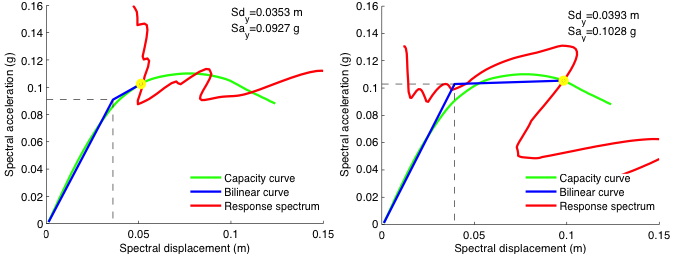
\includegraphics[width=12cm]{Figures/performance_points.png}
  \caption{Assessment of the target displacement for "weak" (left) and "strong" (strong) ground motion record.}
  \label{fig:per_point}
\end{figure}

The initial proposal of this method was heavily criticized due to its tendency to underestimate the deformation of the structures, which was mostly related with the model employed to calculate the equivalent viscous damping (e.g. \cite{Fajfar1999}; \cite{ChopraGoel2010}). Thus, in \cite{FEMA4402005}, some modifications were proposed regarding the calculation of this component. Furthermore, several other models relating an equivalent viscous damping ratio ($\xi_{eq}$) with a ductility level ($\mu$) have been proposed in the last decades, and implemented in the RMTK. The following list describes these models, and specifies the code that must be defined in the variable \verb=damping_model= in order to follow the associated model in the vulnerability calculations.\\

\begin{itemize}
\item \cite{FEMA4402005}: This model assumes different expressions to calculate the equivalent viscous damping ratio depending on the ductility level, hysteretic model and post-elastic stiffness. However, for the sake of simplicity, approximate equations have been proposed to calculate $\xi_{eq}$ with any capacity curve, that only depends on the level of ductility, as described below:\\

For $1.0 < \mu < 4.0$:
\begin{equation}
	\xi_{eq} = \xi_0 + 0.049\left(\mu-1\right)^2-0.01\left(\mu-1\right)^3
\end{equation}

For $4.0 \le \mu \le 6.5$:
\begin{equation}
	\xi_{eq} = \xi_0 + 0.14 + 0.0032 \left(\mu-1\right)
\end{equation}

For $ \mu > 6.5$:
\begin{equation}
	\xi_{eq} = \xi_0 + 0.19\left[\frac{0.64\left(\mu-1\right)-1}{\left[0.64\left(\mu-1\right)\right]^2}\right]\left(\frac{T_{eff}}{T_0}\right)^2
\end{equation}

Where $\xi_0$ stands the initial elastic viscous damping ratio, and $T_{eff}$ represents the effective period, which for ductility above 6.5 can be calculated using the following expression:

\begin{equation}
	T_{eff} = \left\{0.89\left[\sqrt{\frac{(\mu-1)}{1+0.05(\mu-2)}}\right]+1\right\}T_0
\end{equation}

In order to use this model, the variable \verb=damping_model= must be set to \verb=FEMA_2005=.\\

\item \cite{Kowalsky1994}: This model establishes a relationship between the equivalent viscous damping ratio and a ductility level and a post-yield stiffness ratio $\alpha$, as defined by the following equation:

\begin{equation}
\xi_{eq} = \xi_0 + \frac{1}{\pi}\left[1-\frac{(1-\alpha)}{\sqrt{\mu}} - \alpha\sqrt{\mu} \right]
\end{equation}

In order to use this model, the variable \verb=damping_model= must be set to \verb=Kowalsky_1994=.\\

\item \citep{Iwan1980}: This model was developed using a limited number of ground motion records and a single hysteretic model, leading to the following equation:

\begin{equation}
	\xi_{eq} = \xi_0 + 0.0587\left(\mu-1\right)^0.371
\end{equation}

In order to use this model, the variable \verb=damping_model= must be set to \verb=Iwan_1980=.\\

\item \cite{GulkanSozen1974}:This model was derived considering the Takeda hysteretic for elasto-plastic systems calibrated with experimental shaking-table results of a number of reinforced concrete frames. The equivalent viscous damping ratio is calculated using the following ductility-dependent formula:

\begin{equation}
	\xi_{eq} = \xi_0 + 0.2\left(1- \frac{1}{\sqrt{\mu}}\right)
\end{equation}

In order to use this model, the variable \verb=damping_model= must be set to \verb=Gulkan_Sozen_1974=.\\

\item \cite{PriestleyEtAl2007}: These Authors proposed different models depending on the structure type. Currently, three models proposed by this study have been implemented, as described below: \\

For reinforced concrete frame structures:

\begin{equation}
	\xi_{eq} = 0.05 + 0.565\left(\frac{\mu-1}{\pi\mu}\right)
\end{equation}

To use this model set the variable \verb=damping_model= to \verb=Priesley_et_al2007_frames=.\\

For reinforced concrete walls structures:

\begin{equation}
\xi_{eq} = 0.05 + 0.444\left(\frac{\mu-1}{\pi\mu}\right)
\end{equation}

To use this model set the variable \verb=damping_model= to \verb=Priesley_et_al2007_walls=.\\

For steel structures:

\begin{equation}
	\xi_{eq} = 0.05 + 0.577\left(\frac{\mu-1}{\pi\mu}\right)
\end{equation}

To use this model set the variable \verb=damping_model= to \verb=Priesley_et_al2007_steel=.\\

\item \cite{Calvi1999}: This Author proposed a relationship between the equivalent viscous damping ratio and ductility following the expression below:

\begin{equation}
	\xi_{eq} = \xi_0 + a\left(1-\frac{1}{\mu^b}\right)
\end{equation}

Where \verb=a= and \verb=b= are constants that vary between 20 and 30, and 0.5 and 1, respectively, depending on the hysteretic properties of the structure. Thus, this model can be employed for various structure types, by adjusting these two constants. Given the fact that most of the current damping models have been derived or calibrated for reinforced concrete structures, a decision was made to adjust these parameters for the assessment of masonry structures. The \verb=a= and \verb=b= constants have been set to 25 and 0.5, respectively, as proposed by \cite{BorziEtAl2008a}. Nonetheless, due to the open and transparent architecture of the RMTK, any user can modify these parameters.\\

In order to use this model, the variable \verb=damping_model= must be set to \verb=Calvi_1999=.\\

\end{itemize}
The performance point (or target displacement) calculated within this methodology is equivalent to what would be obtained by subjecting the equivalent single degree of freedom oscilator to a nonlinear time history analysis. Then, estimated target displacement can be used to allocate the structure in a damage state, based on a pre-established set of displacement thresholds. This process can be repeated several times considering other ground motion records, as well as structures (i.e. building class).\\

In order to use this methodology, it is necessary to load one or multiple capacity curves and a set of ground motion records, as explained in Section~\ref{subsec:cap_curves} and \ref{subsec:gmrs}, respectively. Then, it is necessary to specify a damage model using the parameter \verb=damage_model= (see Section~\ref{subsec:dmg_model}), and a damping ratio using the parameter \verb=damping=. After importing the module \verb=capacitySpectrumMethod=, it is possible to calculate the distribution of structures across the set of damage states for each ground motion record using the following command:

\begin{Verbatim}[frame=single, commandchars=\\\{\}, samepage=true]
PDM, Sds = capacitySpectrumMethod.calculate_fragility(capacity_curves,...
gmrs,damage_model,damping)
\end{Verbatim}

Where \verb=PDM= (i.e. probability damage matrix) represents a matrix with the number of structures in each damage state per ground motion record, and \verb=Sds= (i.e. spectral displacements) represents a matrix with the maximum displacement (of the equivalent SDoF) of each structure per ground motion record. The variable PDM can then be used to calculate the mean fragility model as described in Section~\ref{subsec:derive_fragility}.



